\chapter{Testování}

Emulátor jakéhokoliv systému který je implementován na základě kusých informací a reverzním inženýrství
bude vždy mít určité nedostatky, nepřesnosti a chyby. Ovšem cílem emulátoru není precizně napodobit chování
emulovaného systému, nýbrž získat \textit{drop-in replacement} za původní systém, kde v případě \textit{PlayStation}
konzole znamená kompatibilitu a hratelnost oficiálně publikovaných her.

Bohužel, přístup k celé \textit{PlayStation} knihovně není pro jednotlivce dost dobře možný. Ty hry, které byly testovány
na tomto emulátoru byly zapůjčeny od blízkých přátel. Samozřejmě testování jednotlivých her je velmi časově náročná
záležitost, neboť na \textit{PlayStation} systém vycházely hry, které vyžadovaly až stovky hodin investice.

\section{Kompatibilita dostupných her}

Z celkem 8 testovaných her, 5 z nich bylo \textit{hratelných}. To znamená, že hráč se dostal přes úvodní intra do hlavní
herní smyčky a měl možnost ovládat to, co se děje na obrazovce (to ovšem neznamená, že hra běžela perfektně, ani že byla dohratelná). Zbytek, který \textit{hratelný} nebyl většinou závisel na specifických 
nedokončených implementací jednotlivých hardwarových komponent (především \textit{CDROM}, \textit{SPU} a \textit{GTE}).
Pro demonstraci jsem zvolil 3 různé dostupné hry, které byly \textit{hratelné}.

\subsection{Skullmonkeys}

Tato hra, při testování byla \textit{hratelná} od začátku až do konce. Jde o zástupce 2D \textit{PlayStation} her
a tedy testovala schopnosti emulátoru správně vykreslovat texturované a obarvené obdélníky, viz obrázky \ref{skullmonkeys-showcase-1} a \ref{skullmonkeys-showcase-3}.
Hra ovšem neběžela bez problémů. Její koncept je budován na základě skrolovaných úrovní a v určitých částech
hra načítala stavební bloky úrovně příliš pozdě, jak můžeme vidět v obrázku \ref{skullmonkeys-showcase-2}. Co tento nedostatek způsobilo není známé, ovšem
s nejvyšší pravděpodobností jde o špatně načasované přerušení, nebo hře je poskytována špatná hodnota
ohledně pozice kamery (možná špatná znaménková interpretace registru v \textit{GPU} nebo \textit{GTE}). 

\subsection{Final Fantasy VII}

Tato hra byla bohužel příliš dlouhá\footnote{\url{https://howlongtobeat.com/game/3521}} na otestování všech kapabilit,
nicméně zhruba 2-hodinová seance běžela bez větších problémů. Tato hra kombinuje 3D modely s 2D pozadím dekódované pomocí čipu \textit{MDEC} vytvářející
iluzi 3D scény. Výjimkou jsou bitevní scény, které plně využívají 3D schopností \textit{PlayStation} systému, viz obrázky \ref{ff7-showcase-1} a \ref{ff7-showcase-3}. Ukázal se ovšem minoritní problém
při vykreslování polygonů, kde tato hra při vykreslování 2D pozadí využívá zelenou masku, pomocí níž filtruje 3D modely, aby se správně scéna zobrazila.
Tato zelená maska by teoreticky neměla být nikdy vidět, ovšem může se stát že se sem tam nějaký ten pixel nepřesně vykreslí, jak si můžeme všimnout v obrázku \ref{ff7-showcase-2}.
Tento nedostatek může být způsoben špatnou interpolací atributů vrcholů trojúhelníku, nebo je špatně logika \textit{fixed-point} aritmetiky
kterou \textit{GPU} rasterizace používá.

\subsection{Ghost in the Shell}

Tato hra používá širokou škálu \textit{GTE} příkazů a tedy řádně tuto hardwarovou komponentu otestovala.
Až na výjimečné chyby v texturování trojúhelníků a občasné zaseknutí emulátoru, tato hra běžela relativně dobře, viz obrázky \ref{gits-showcase-1} a \ref{gits-showcase-2}.

\section{Měření/Potenciální optimalizace}

Bezpochyby přesnost emulace může mít zásadní vliv na hratelnost jednotlivých her. Ovšem pokud se emulace vleče,
celkový požitek ze hry může být tímto faktorem narušen. Měření rychlosti bylo provedeno jako násobek odchylky od
ideálního běhu emulátoru. To znamená, že pokud konzole vyžadovala \textit{50} snímků za sekundu, ale emulátor při plné
rychlosti dokázal simulovat \textit{100} snímků za sekundu, výsledek měření by byl \textit{2}, protože emulátor
dokáže simulovat systém s dvojnásobnou rychlostí. Výsledek měření je zachycen v grafu \ref{cpu-performance}.

Vzhledem k tomu, že celková architektura tohoto emulátoru byla navržena spíše pro modularitu a celkovou čitelnost zdrojového kódu, 
rychlostně tento emulátor poněkud tápe. Ovšem existují hlavní místa, ve kterých by se dalo získat nemálo procesorových cyklů popsané v sekcích [\ref{cpu-optimizations}] a [\ref{gpu-optimalization}].

\subsection{Potenciální optimalizace CPU} \label{cpu-optimizations}

\textit{CPU} modul v současné době je řešen čistě jako interpretace proudu \textit{MIPS} instrukcí.
Ovšem existuje rychlejší a mnohem složitější varianta jak transformovat jednu instrukční architekturu na architekturu jinou.
Tím samozřejmě myslím koncept \textit{Just In Time (JIT)} kompilace, či \textit{rekompilátor}, který by za běhu dokázal identifikovat
bloky instrukcí a transformovat je na nativní sekvenci instrukcí hostovacího systému. V našem případě by se
jednalo o \textit{MIPS R3000A} na \textit{x86\_64} \textit{rekompilátor}. Výsledný transformovaný blok by se pak nativně
zavolal a tím by se dalo získat nemálo procesorových taktů.

Ačkoliv jednoduchý \textit{JIT} modul by nebylo příliš složité na implementaci, tento koncept vyžaduje hlubokou znalost obou instrukčních sad
a celkově se jedná o velmi časově náročnou záležitost. \textit{JIT} taky znamená poteciální risk co se bezpečnosti týče,
protože \textit{JIT} vyžaduje vytváření spustitelného bloku v paměti za běhu, který přímo byte po bytu modifikujeme.

\subsection{Potenciální optimalizace GPU} \label{gpu-optimalization}

V \textit{GPU} probíhá veškerá rasterizace softwarově pomocí hostovacího \textit{CPU}. Potenciální zrychlení by se dalo nalézt v hardwarové rasterizaci
pritiv. Je ovšem na pováženou jak moc by hardwarová rasterizace v základním režimu pomohla, protože většina 3D scén, které se \textit{PlayStation} hry
snaží vykreslit, jsou vesměs velmi malé trojúhelníky a jejich počet se pohybuje kolem spodních tisíců (nejnáročnější z testovaných her byla \textit{Ghost in the Shell}, kde za běhu hry bylo naměřeno až 3000 vykreslených trojúhelníků za jeden snímek). S takto malou pracovní jednotkou
není jisté, zda-li samotná práce s hostovacím \textit{GPU} (především přenos dat z a do hostovacího \textit{GPU}) by nezabíralo více času, než softwarové renderování. Tato spekulace samozřejmě padá při renderování ve vyšším rozlišení, kde hardwarový renderer by naprosto jistě zrychlil celý chod emulátoru.

\begin{figure}[hbt]
    \centering
    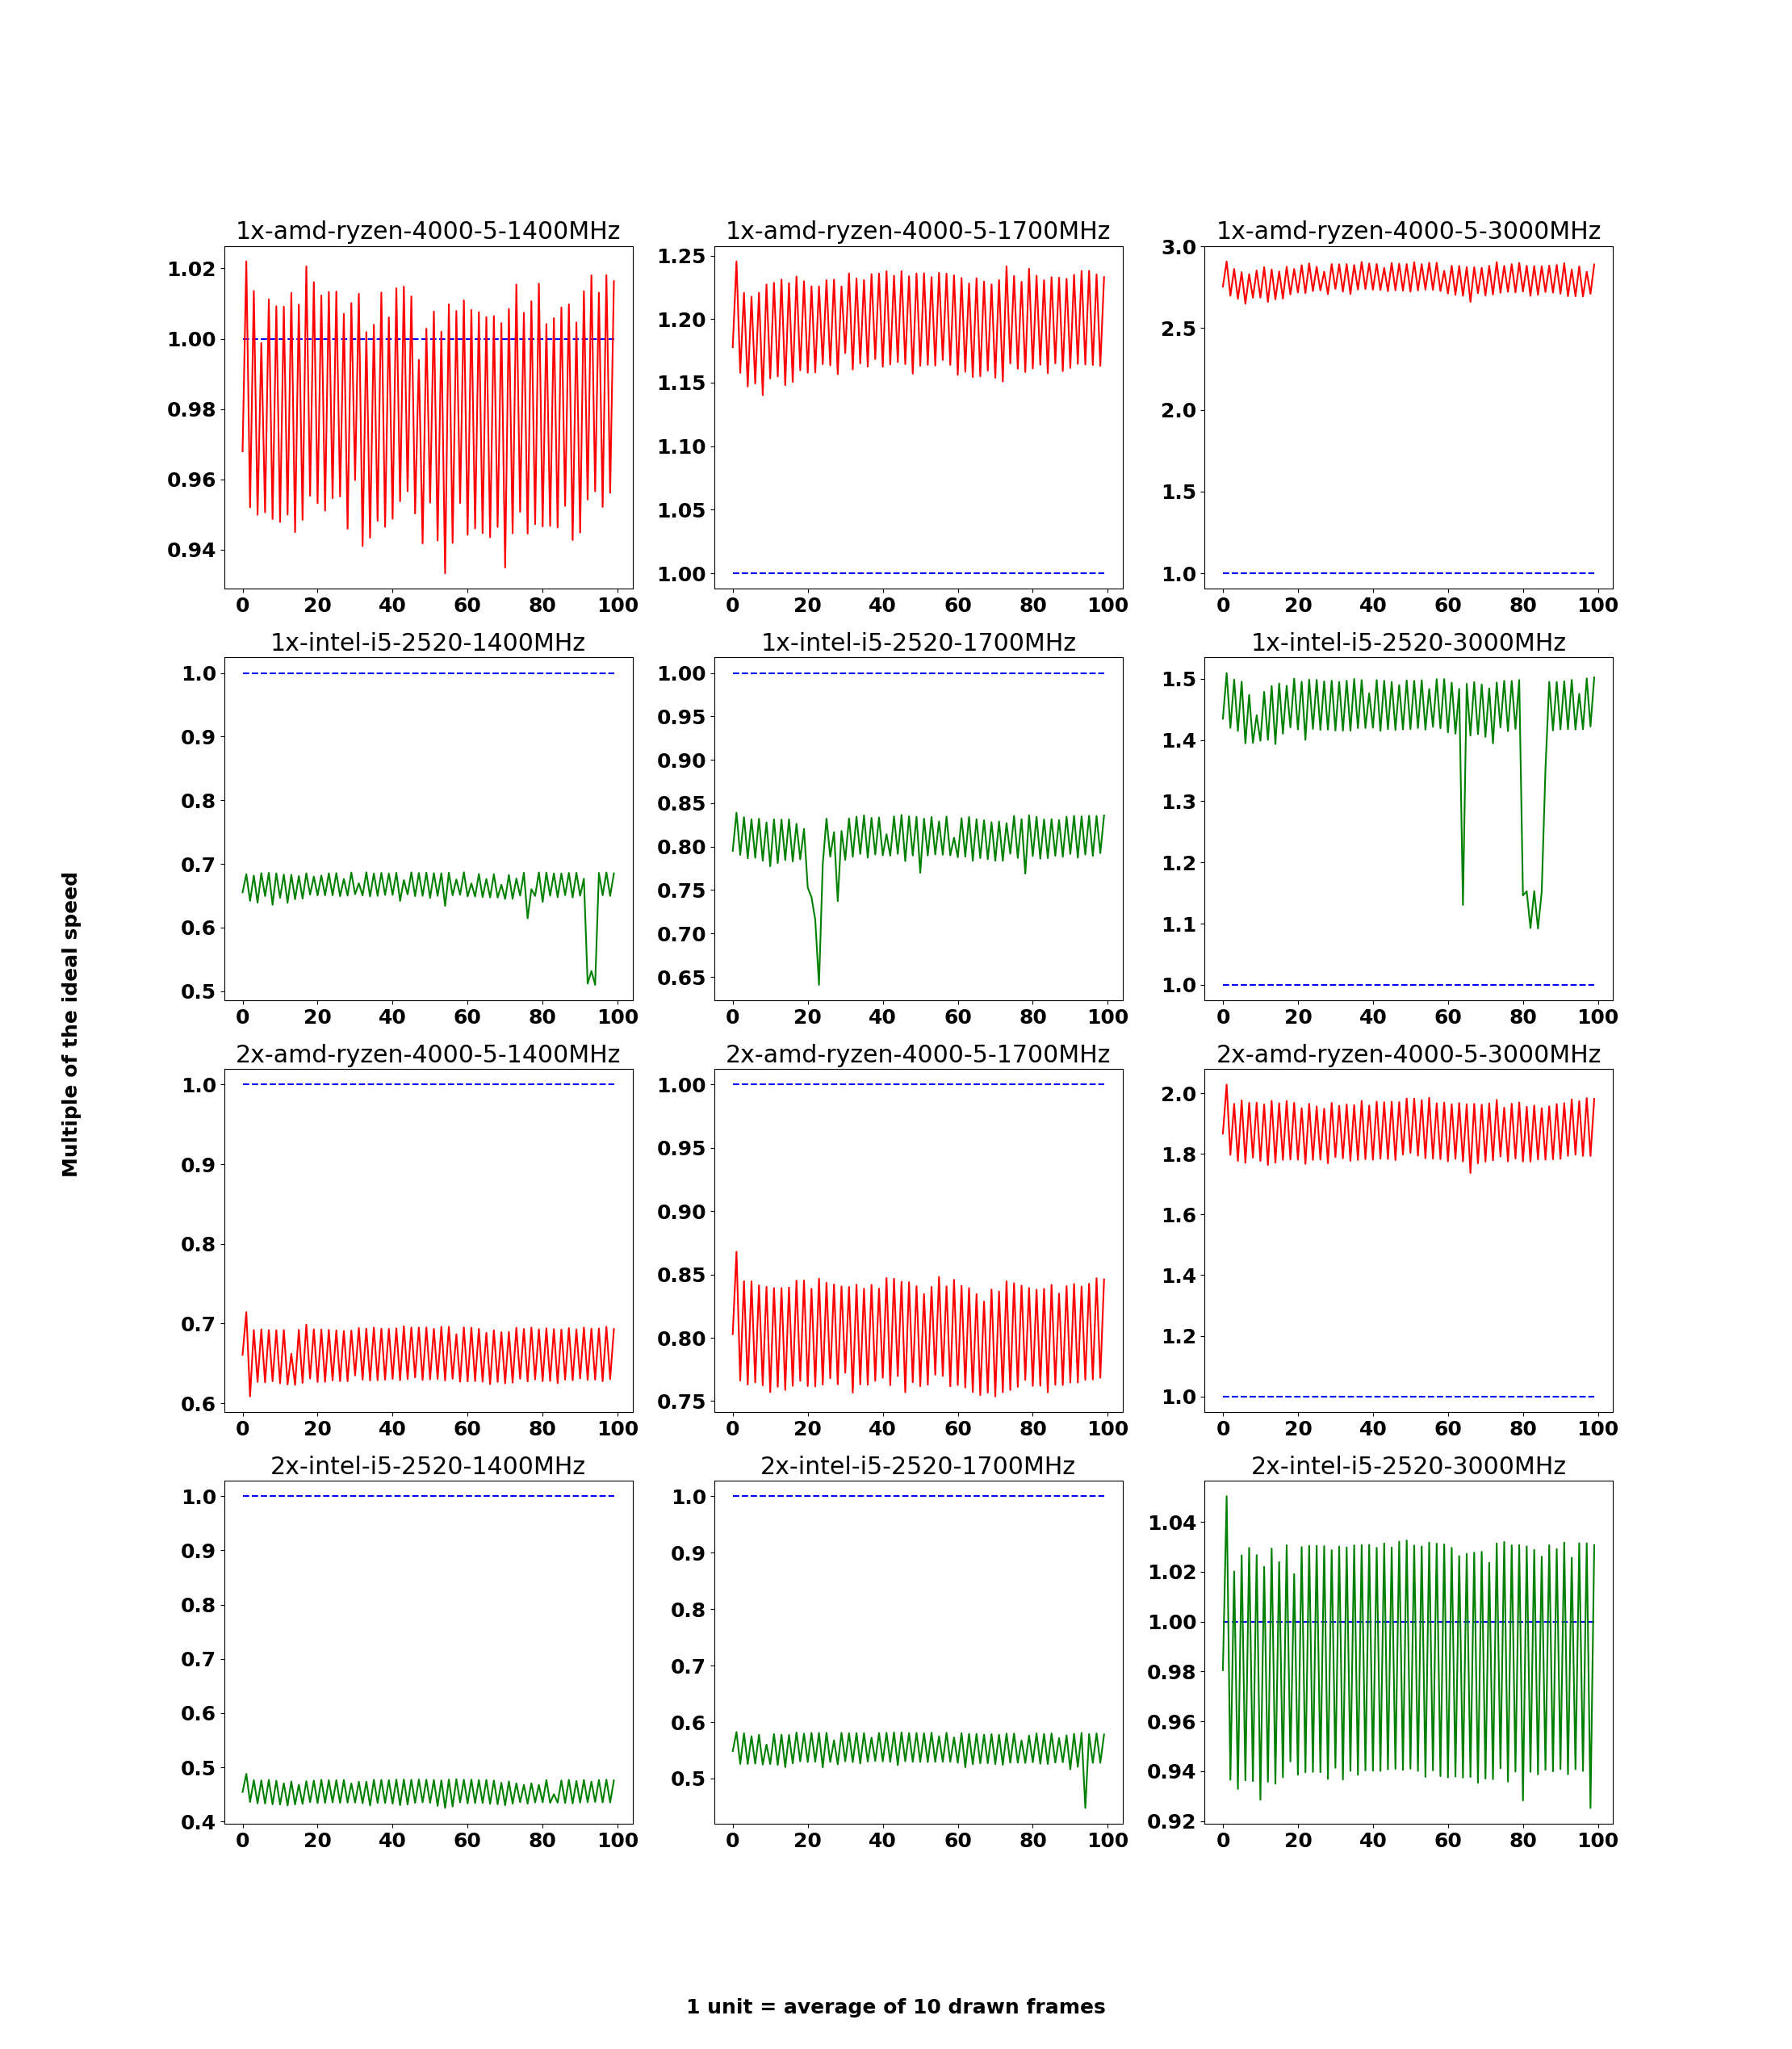
\includegraphics[width=1.0\textwidth]{obrazky-figures/cpu-performance.png}
    \caption[Performanční graf]{Rychlost emulace především závisí na schopnostech hostovacího procesoru. Testovány byly dva různé procesory (
    \textbf{\color{red}AMD 4000 5 - červený graf} a \textbf{\color{green}intel i5 2520 - zelený graf}). V každém z grafu
    je také přerušovaná \textbf{\color{blue}ideální čára}, která slouží jako referenční bod ideálního běhu emulátoru.
    Pokud graf je nad touto přerušovanou čárou, znamená to, že hostovací procesor dokáže \textit{PlayStation} systém simulovat rychleji.
    Stejně tak pokud graf je pod přerušovanou čárou, emulátor nestíhá simulovat systém dostatečně rychle.
    Graf tedy zobrazuje násobek ideální rychlosti vzhledem k indexu naměřeného snímku (horizontální osa), přičemž prefix názvu grafu určuje, při jakém násobku rozlišení bylo měření provedeno (\textbf{1x} a \textbf{2x}).
    Oba procesory byly postupně omezeny vzhledem k jejich hodinové rychlosti. U tohoto porovnání procesorů si můžeme všimnout, že čistě rychlost hodin není všechno. \textbf{\color{red}AMD 4000 5} disponuje \textit{3MiB L2 cache} a \textit{8 MiB L3 cache}, kdežto \textbf{\color{green}intel i5 2520} má pouze \textit{512 KiB L2 cache} a \textit{3 MiB L3 cache}. Naměřená data se nacházejí v přílohách \ref{amd-ryzen-perf} a \ref{intel-perf}}.
    \label{cpu-performance}
\end{figure}

\begin{figure}[hbt]
    \begin{subfigure}{0.5\textwidth}
        \centering
        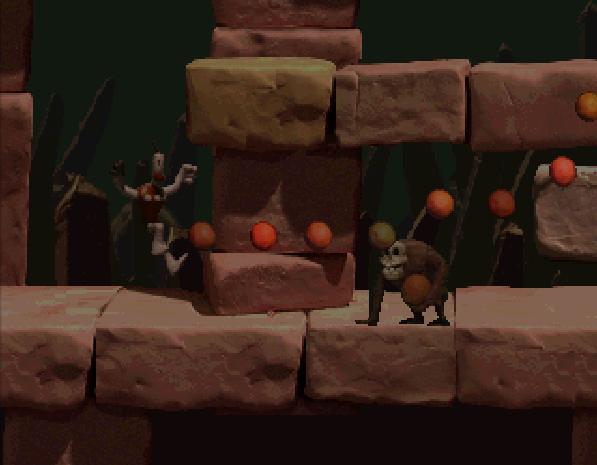
\includegraphics[width=0.9\textwidth, height=6cm]{obrazky-figures/skullmonkeys-showcase-1-1.png}
    \end{subfigure}
    \begin{subfigure}{0.5\textwidth}
        \centering
        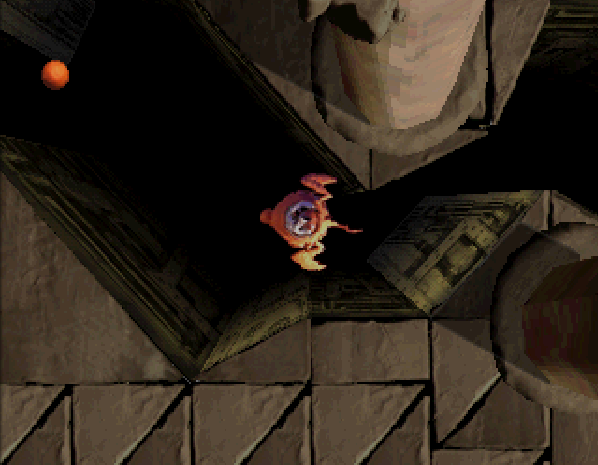
\includegraphics[width=0.9\textwidth, height=6cm]{obrazky-figures/skullmonkeys-showcase-1-2.png}
    \end{subfigure}
    \caption[Test hry \textit{Skullmonkeys}]{Ačkoliv \textit{Skullmonkeys} je dominantně 2D skákačka, hra obsahuje určité úrovně, v nichž utilizuje 3D schopnosti \textit{PlayStation} systému.}
    \label{skullmonkeys-showcase-1}
\end{figure}

\begin{figure}[hbt]
    \begin{subfigure}{0.5\textwidth}
        \centering
        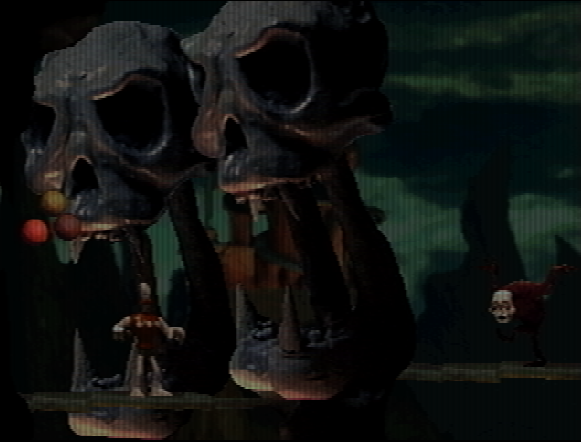
\includegraphics[width=0.9\textwidth, height=6cm]{obrazky-figures/skullmonkeys-showcase-2-1.png}
    \end{subfigure}
    \begin{subfigure}{0.5\textwidth}
        \centering
        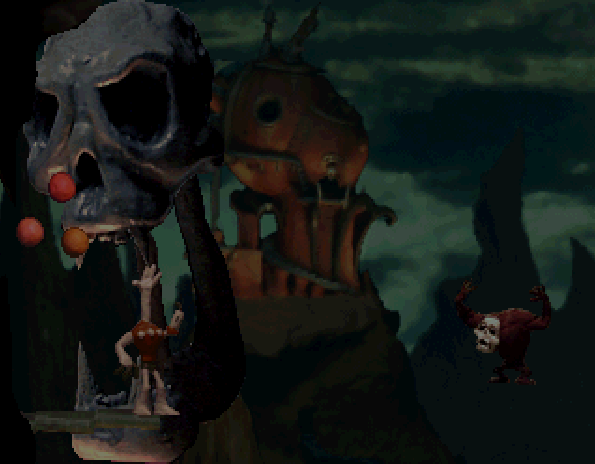
\includegraphics[width=0.9\textwidth, height=6cm]{obrazky-figures/skullmonkeys-showcase-2-2.png}
    \end{subfigure}
    \caption[Nedostatky ve hře \textit{Skullmonkeys}]{Vlevo si můžeme všimnou správně vykreslené úrovně (emulátor \textit{SwanStation}) a napravo je současný stav mého emulátoru, kde chybí části úrovně.}
    \label{skullmonkeys-showcase-2}
\end{figure}

\begin{figure}[hbt]
    \begin{subfigure}{0.5\textwidth}
        \centering
        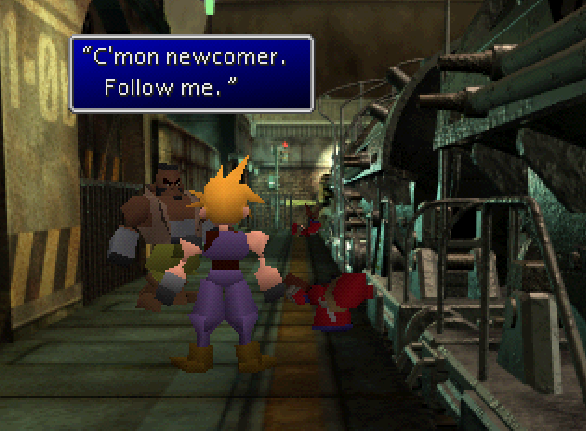
\includegraphics[width=0.9\textwidth, height=6cm]{obrazky-figures/ff7-showcase-1-1.png}
    \end{subfigure}
    \begin{subfigure}{0.5\textwidth}
        \centering
        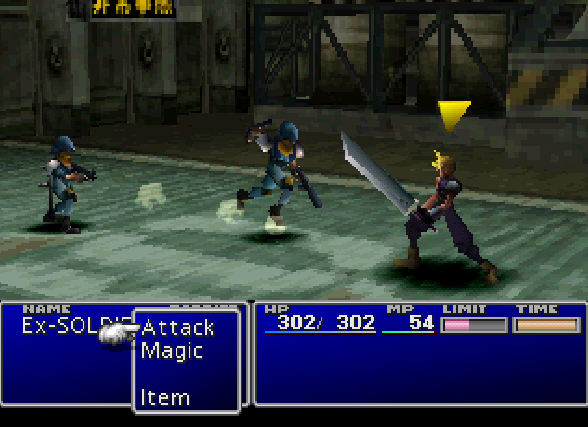
\includegraphics[width=0.9\textwidth, height=6cm]{obrazky-figures/ff7-showcase-1-2.png}
    \end{subfigure}
    \caption[Test hry \textit{Final Fantasy VII}]{Vlevo si můžeme všimnou kombinace předem vyrendrovaného 2D pozadí, které v kombinaci s 3D modely dokázaly vytvořit solidní iluzi 3D prostředí. Vpravo pak
             vidíme plně 3D vykreslenou dynamickou scénu.}
    \label{ff7-showcase-1}
\end{figure}

\begin{figure}[hbt]
    \begin{subfigure}{0.5\textwidth}
        \centering
        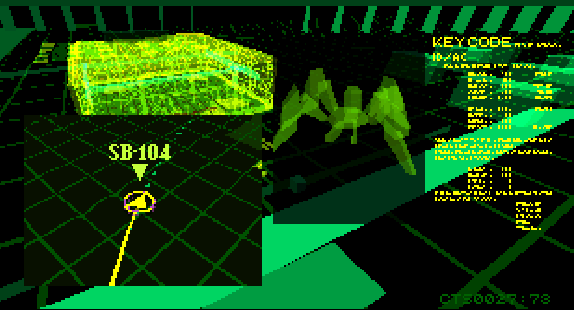
\includegraphics[width=0.9\textwidth, height=6cm]{obrazky-figures/gits-showcase-1.png}
    \end{subfigure}
    \begin{subfigure}{0.5\textwidth}
        \centering
        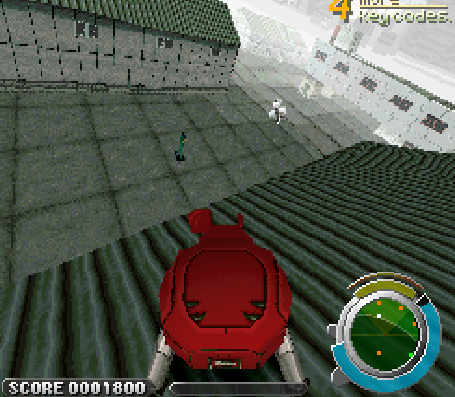
\includegraphics[width=0.9\textwidth, height=6cm]{obrazky-figures/gits-showcase-2.png}
    \end{subfigure}
    \caption[Test hry \textit{Ghost in the Shell}]{Briefing mise, který vidíme v levém obrázku, vyžaduje dobré pokrytí většiny příkazů \textit{GTE} komponenty.
    Stejně tak hlavní herní smyčka, v obrázku v pravo, provádí netriviální transformace scény.}
    \label{gits-showcase-1}
\end{figure}

\begin{figure}[hbt]
    \begin{subfigure}{0.5\textwidth}
        \centering
        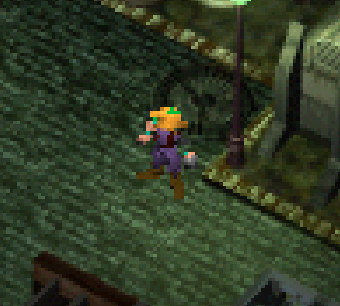
\includegraphics[width=0.9\textwidth, height=6cm]{obrazky-figures/ff7-showcase-2-1.png}
    \end{subfigure}
    \begin{subfigure}{0.5\textwidth}
        \centering
        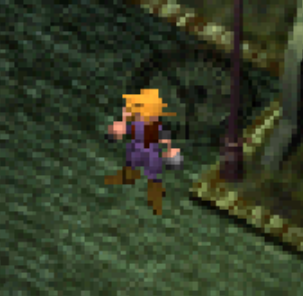
\includegraphics[width=0.9\textwidth, height=6cm]{obrazky-figures/ff7-showcase-2-2.png}
    \end{subfigure}
    \caption[Nedostatky ve hře \textit{Final Fantasy VII}]{Z neznámeho důvodu, příliš malé trojúhelníky se v mém emulátoru nevykreslují korektně, nebo jde o chybu při interpolaci barev vrcholů. Tento artefakt je
     patrný v levém obrázku, kde zelená maska, použitá pro správné vykreslení 2D pozadí, se "propíjí" do 3D modelů.}
    \label{ff7-showcase-2}
\end{figure}

\begin{figure}[hbt]
    \centering
    \begin{subfigure}{0.9\textwidth}
        \centering
        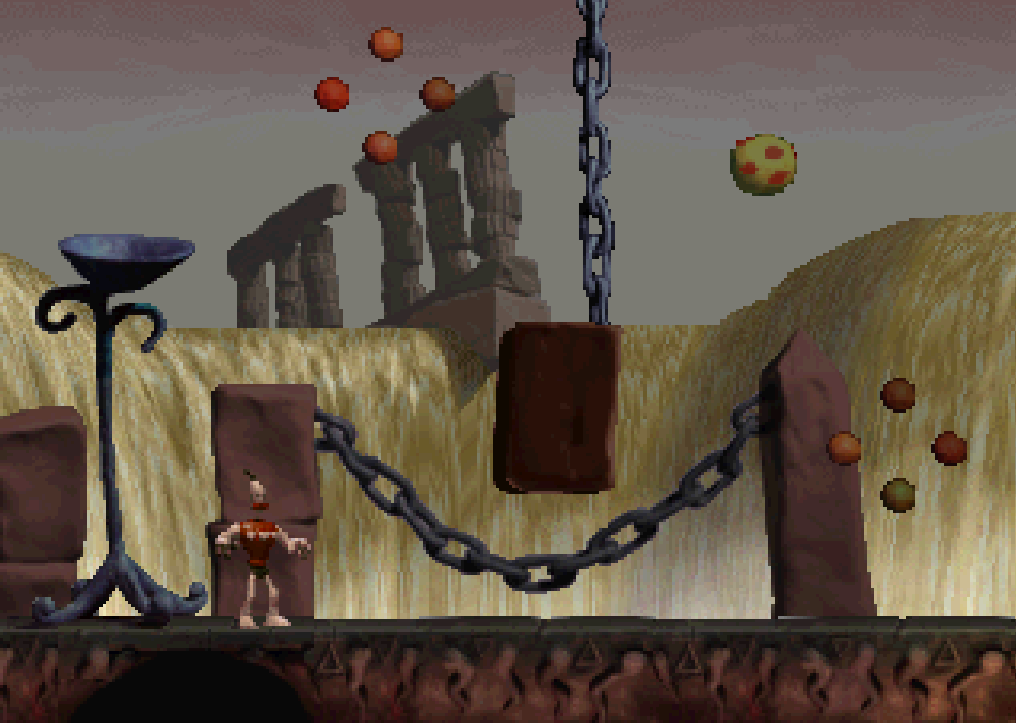
\includegraphics[width=0.9\textwidth, height=10cm]{obrazky-figures/skull-lowres.png}
        \vspace*{2mm}
    \end{subfigure}
    \begin{subfigure}{0.9\textwidth}
        \centering
        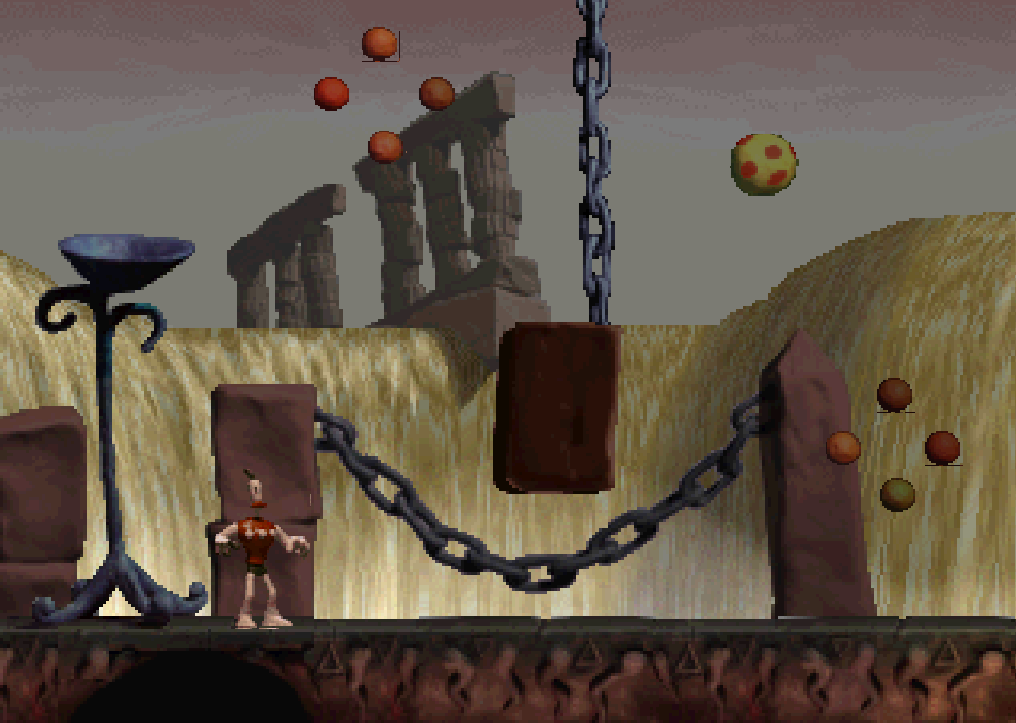
\includegraphics[width=0.9\textwidth, height=10cm]{obrazky-figures/skull-highres.png}
    \end{subfigure}
    \caption[Změna rozlišení u hry \textit{Skullmonkeys}]{Při zvýšení rozlišení se textury úrovně příliš nezmění, ale můžeme si povšimnout změny vykreslení dynamických objektů. V této scéně jsou objekty, jako například hlavní postavička, zmenšeny. Pokud ale zvýšíme rozlišení, dynamické objekty získají zpět svůj detail.}
    \label{skullmonkeys-showcase-3}
\end{figure}

\begin{figure}[hbt]
    \centering
    \begin{subfigure}{0.9\textwidth}
        \centering
        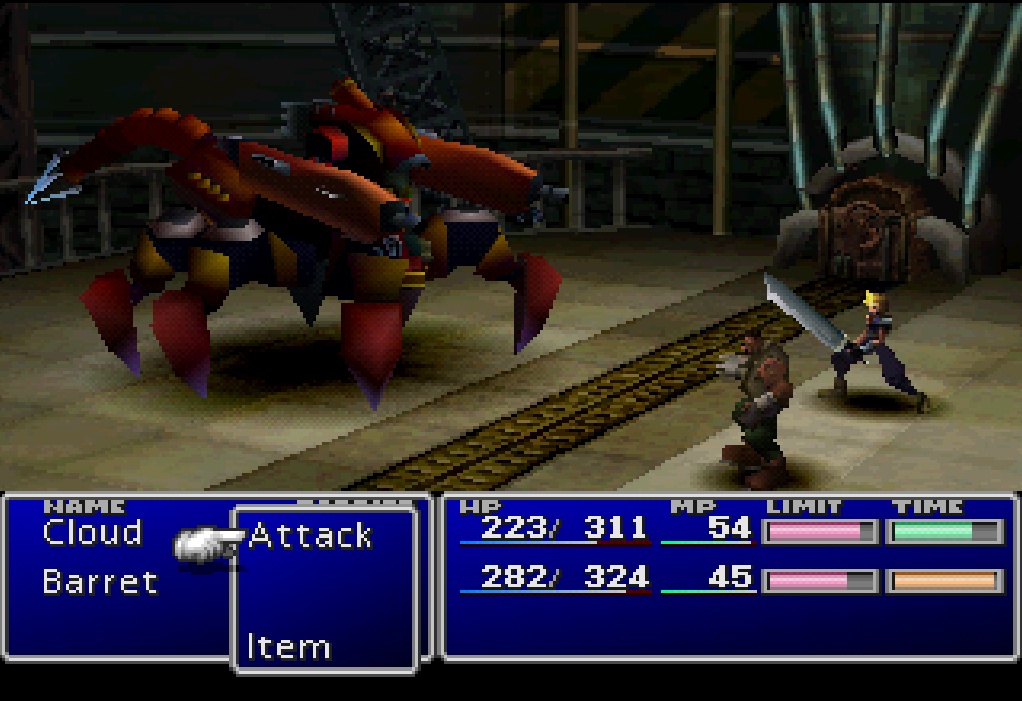
\includegraphics[width=0.9\textwidth, height=10cm]{obrazky-figures/ff7-lowres.png}\vspace*{2mm}
    \end{subfigure}
    \begin{subfigure}{0.9\textwidth}
        \centering
        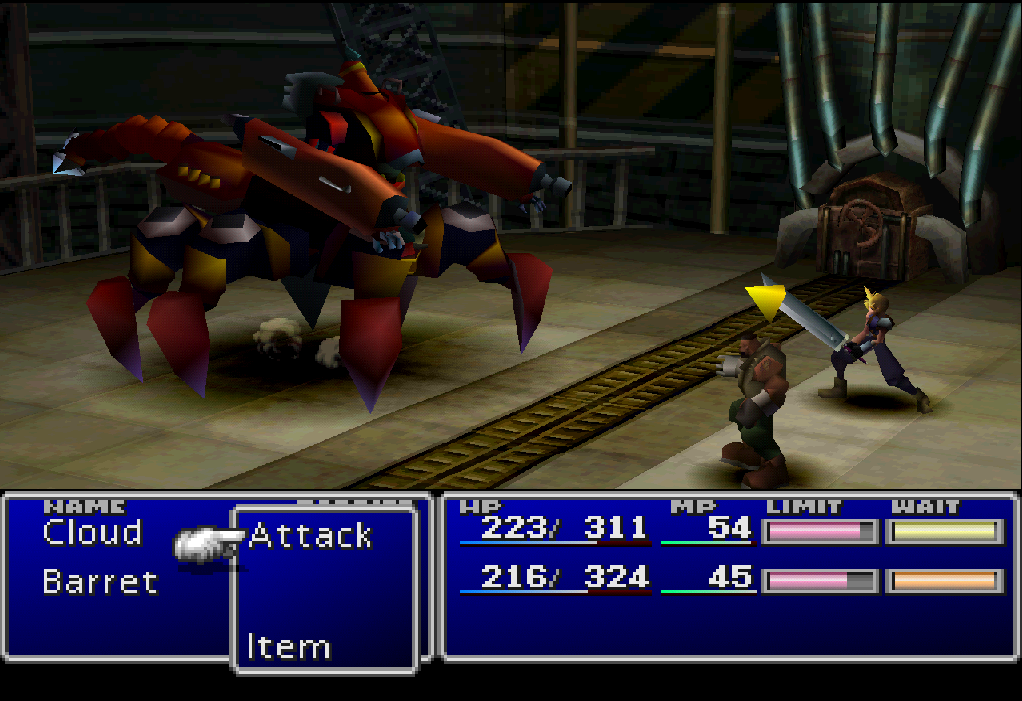
\includegraphics[width=0.9\textwidth, height=10cm]{obrazky-figures/ff7-highres.png}
    \end{subfigure}
    \caption[Změna rozlišení u hry \textit{Final Fantasy VII}]{Ačkoliv při změně rozlišení textury menu zůstávají stále hranaté, samotná scéna získává úplně nový nádech.}
    \label{ff7-showcase-3}
\end{figure}

\begin{figure}[hbt]
    \centering
    \begin{subfigure}{0.9\textwidth}
        \centering
        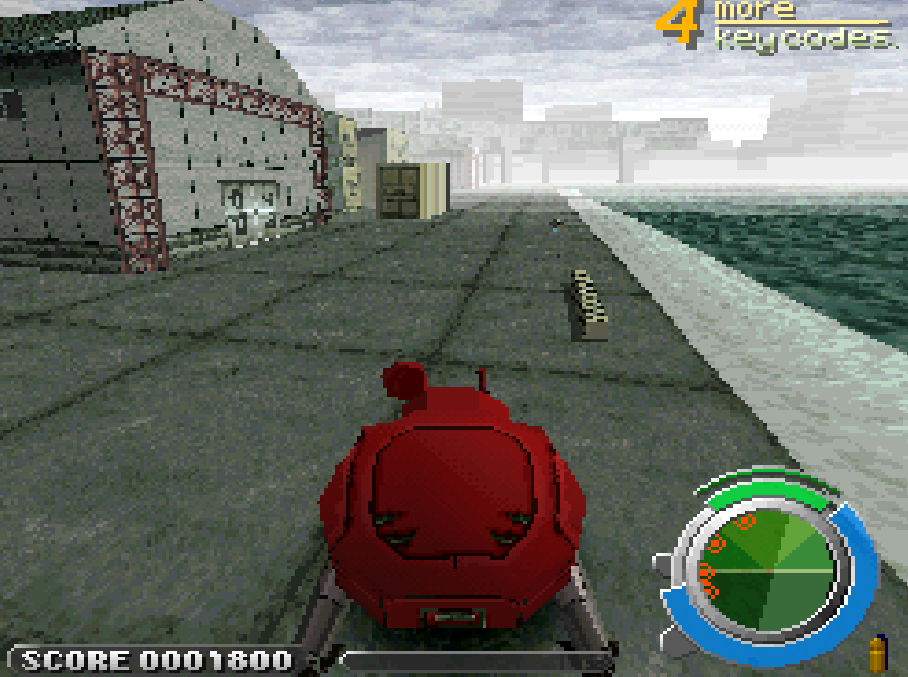
\includegraphics[width=0.9\textwidth, height=10cm]{obrazky-figures/gits-lowres.png}
        \vspace*{2mm}
    \end{subfigure}
    \begin{subfigure}{0.9\textwidth}
        \centering
        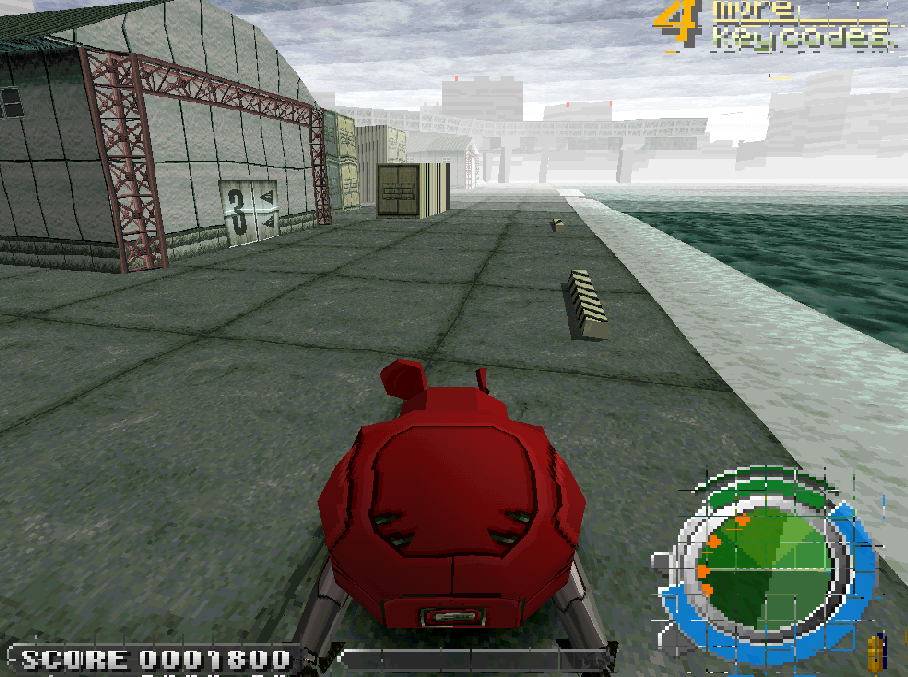
\includegraphics[width=0.9\textwidth, height=10cm]{obrazky-figures/gits-highres.png}
    \end{subfigure}
    \caption[Změna rozlišení u hry \textit{Ghost in the Shell}]{ Při změně rozlišení se stává, že obdélníková primitiva mají malý problém s adresováním textur. Radar v pravém dolním rohu obrazovky obsahuje viditelné \textit{jizvy}. Můžeme si také všimnout, že změna rozlišení nám snadněji dovolí rozpoznávat vzdálené objekty, jako například číslo 3 na dveřích budovy v levé části obrázku. }
    \label{gits-showcase-2}
\end{figure}